\section{Конструкторская задача}

Спроектировать захватывающе-сбрасывающее устройство для коптера, на котором будет осуществляться перемещение груза размерами 7-10 см и массой 60-80 грамм. Для проектирования использовать Autodesk Inventor (или любое другое ПО для создания CAD-моделей). По окончании проектирования и тщательной проверки модели на предмет совпадения размеров распечатать захватывающее устройство (или его элементы в зависимости от конструкции) на 3D принтере, собрать полученное изделие и протестировать на коптере с грузом. 

\textbf{Готовый результат выполненной задачи} — собранное захватывающе-сбрасы-вающее устройство, протестированное и выполняющее задачи перемещения груза без повреждения груза и коптера.  

\subsubsection*{Пример решения}

В качестве груза проще всего сделать небольшой куб, на который после печати можно будет прикрепить металлическую наклейку:

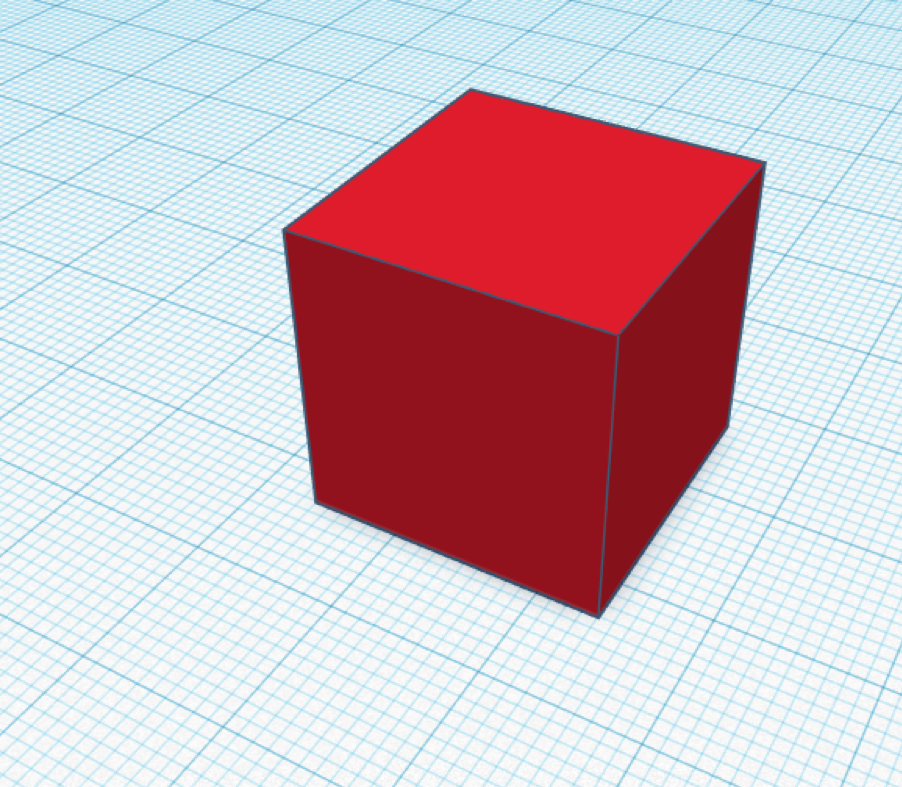
\includegraphics[width=15cm]{final/command_tour/ats/task_09/1.png}

А в качестве захватывающего устройства используется электромагнит, соответственно необходимо прикрепить его к коптеру:

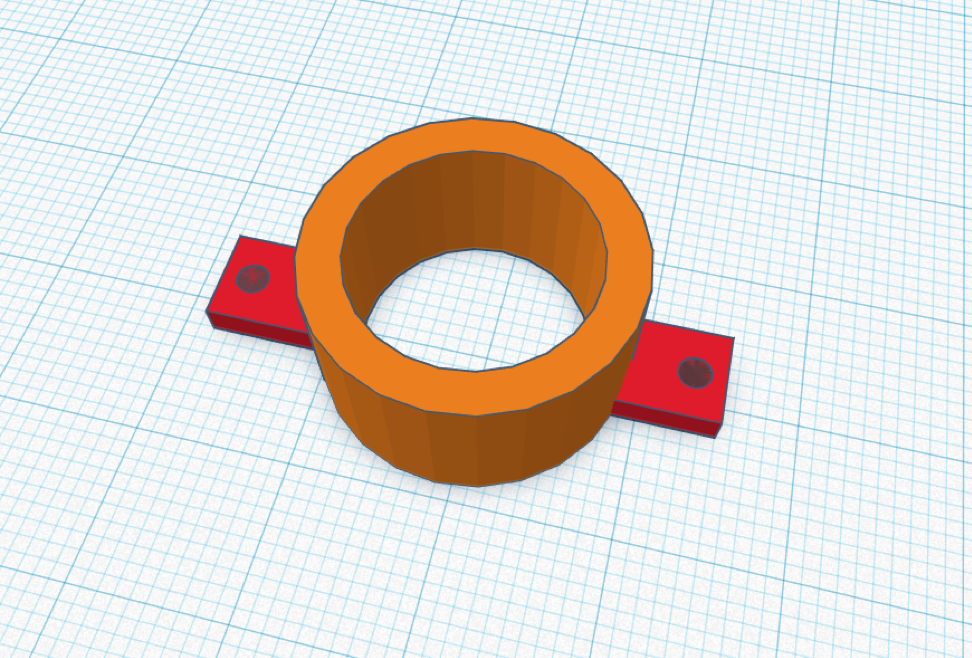
\includegraphics[width=15cm]{final/command_tour/ats/task_09/2.png}

